% AUTHOR: ASHWIN ABRAHAM

\documentclass[12pt]{report}
\usepackage[a4paper, total={6in, 8in}]{geometry}
\usepackage{xcolor}
\usepackage{amsmath}
\usepackage{amsfonts}
\usepackage{algpseudocode}
\usepackage{mathtools}
\usepackage{xcolor}
\usepackage{float}
\usepackage{framed}
\usepackage{listings}
\lstset{basicstyle=\ttfamily,
  commentstyle=\color{red},
  keywordstyle=\color{blue},
  %basicstyle=\footnotesize,
  frame=lines,
  numbers=left,
  stepnumber=1,
  showstringspaces=false,
  tabsize=1,
  breaklines=true,
  breakatwhitespace=false,
}
\usepackage{hyperref}
\hypersetup
{
    colorlinks=true,
    linkcolor=blue,
    filecolor=magenta,
    urlcolor=cyan,
    pdftitle={\Huge \textbf{Reinforcement Learning}},
    pdfpagemode=FullScreen,
}
\usepackage[utf8]{inputenc}
\usepackage{graphicx}
\usepackage{longtable}
\usepackage{multirow}


\title{\Huge \textbf{Winter of Data Science Report} \\ on \\ \textbf{Reinforcement Learning}}
\author{\Large Ashwin Abraham}
\date{\Large December 18th, 2022}

\begin{document}
\begin{titlepage}
    \maketitle
\end{titlepage}

\tableofcontents
\newpage

\chapter{Introduction to Reinforcement Learning}
\section{What is Reinforcement Learning?}
Reinforcement Learning is a type of Machine Learning where an agent learns to interact with it's environment in such a way as to maximize a reward signal.
The agent is not told which actions are the best, but must learn this itself by trial and error.

\section{Some Terminology}
\begin{itemize}
    \item The environment of the agent is characterized by it's \textbf{state}.
    \item The agent can take \textbf{actions} in order to modify the state.
    \item An action is taken by our agent every \textbf{timestep}.
    \item The state of the environment may change without any action from the agent (for example in two player games, where the other player is modelled as part of the environment).
    \item Every \textbf{timestep}, our agent takes an action and gets a \textbf{reward} based on the previous state and the action chosen.
    \item The goal of our agent is to learn a \textbf{policy/strategy} (a mapping from state to action) that maximizes the \textbf{total reward} the agent recieves.
    \item The \textbf{value} of a state is a measure of the maximum possible reward the agent can accumulate that state. For games that don't terminate, we can
    define the value of a state as the average reward per unit time that the agent can acquire from that state. In this situation it is clear that we are better of with a policy that chooses the 
    action leading to the state of the highest value, and not the action with the highest reward.
\end{itemize}
In general, all of these may be stochastic and may change with time.

We have not defined any of these formally yet, and we shall revisit all these terms and define them when we learn about \textbf{Markov Decision Processes}, which are used to formally frame the Reinforcement Learning Problem.

\section{Exploration vs Exploitation}
The conflict between \textbf{exploration} and \textbf{exploitation} is one of the most challenging aspects of Reinforcement Learning.
The problem arises due to the fact that we do not know neither the rewards associated with each action nor the value of each state beforehand.
We can only estimate these from the rewards obtained so far.

To improve our estimates, we must try out all states, even the ones with low estimated rewards. This is known as \textbf{exploration}.
However, we must also try to maximize the reward that we collect. Also, it is more important to know precisely the values of the higher value states than those of the lower value ones. 
To do this, we have to move to the states with the highest values. This is known as \textbf{exploitation}.
Naturally, the two conflict with each other. 

A large part of Reinforcement Learning is just finding creative ways of balancing exploration and exploitation.

\section{Classical Methods}
One situation where Reinforcement Learning is commonly used is in training an algorithm to play games. We shall soon look at Reinforcement Learning Algorithms that learn
to play games. However, it is important to note that there are many classical ways of finding algorithms to win such games as well. Let us look at a few examples.
\subsection{Game Trees}

Let us look at two player \textit{perfect information}\footnote{Each player knows the entire state of the game at every stage} \textit{zero-sum}\footnote{If we associate to each outcome of the game a gain for each player (each player aims to maximize their gain), then for each outcome the sum of gains over all players is constant (taken to be $0$ by convention). In the two player case, this means that each game either ends with a win for one player and a loss for the other or with a draw.} turn based finite games, such as Tic-Tac-Toe, Chess, etc. Each of these games ends in either a win for a player and a loss for the other or in a draw.

We can create a structure known as a game tree, which is a tree linking all the possible states the game can find itself in.
Here each state corresponds to a node in the tree, with the starting position as the root. The children of each node correspond to the states reachable from the original node's state.
\begin{figure}[H]
    \centering
    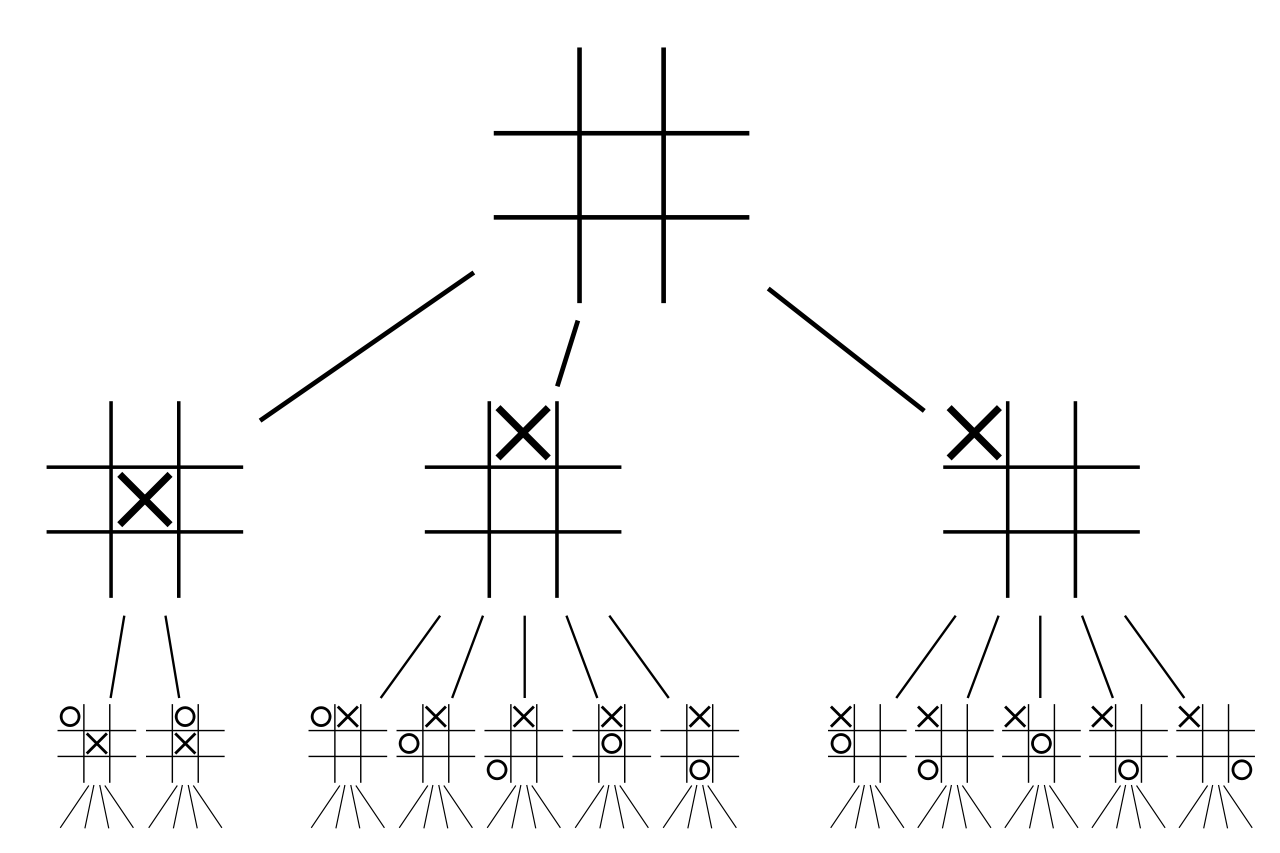
\includegraphics[width=0.6\textwidth]{images/tic_tac_toe_game_tree.png}
    \caption{The first three levels of the game tree of Tic Tac Toe (upto symmetry)}
\end{figure}

Ideally, states should appear in pairs in the game tree, depending on which players turn it is to play. However, for multiplayer games where the players alternate in turns to play, we
can identify the player if we know who the first player was and how many turns have passed since the game started. So in our tree, we do not need to have multiple copies of states differing only in player.

For two player turn based terminating games, in order to make the arguments less verbose, let us call the player who started the game \textbf{Player A}, and the other player, \textbf{Player B}.
However, in any state, let us call the player whose turn it is to play, \textbf{Player 1} and the other player, \textbf{Player 2}. The introduction of these terms makes the arguments less verbose.
However, it is important to note that the identities of players 1 and 2 are not fixed and keep going back and forth between players A and B every turn.

Any game played corresponds to a path from the root of the tree to a leaf. At the root, player 1 is player A and player 2 is player B. As we go down the tree from one node to the next, the identities of players 1 and 2 keep getting swapped.
Now, a leaf node must be either a win for the player 1 (a loss for player 2) or a loss for player 1 (a win for player 2) or a draw.
Let us assign the leaf nodes a value of $0$ if they correspond to draws, $1$ if player 1 has won, and $-1$ if player 1 has lost. 

In general, we assign a value of $1$ to a node, if player 1 has a winning strategy, $0$ if player 1 has no winning strategy, but can force a draw, and $-1$ if no matter what player 1 does, player 2 can play in such a way as to win.

Now, if all the children of a node have value $1$, this means that no matter what player whose turn it is does, he moves into a state where the other player has a winning strategy.
Therefore, this state is losing for the player, ie, it has value $-1$. On the other hand, if there exists a child state with value $-1$, then there exists a move that the player can make
that puts the other player in a losing position, ie, the original state has value $1$. If there exists no child state with value $-1$ but a child state with value $0$, then the player does not have 
a winning strategy but can force a draw. Hence this state has value $0$.

Now, we can find the values of every node in the tree from the bottom up, according to the relation:
\begin{equation}
    V(u) = \begin{cases}
        1, & \exists v \in C(u): V(v) = -1\\
        0, & \forall v \in C(u): V(v) \geq 0, \exists v \in C(u): V(v) = 0 \\
        -1, & \forall v \in C(u): V(v) = 1
    \end{cases}
\end{equation}
Here $V(u)$ represents the value of a node $u$, and $C(u)$ represents the set of children of $u$.

From, this we can conclude that every node in the tree has a value of either $-1$, $0$ or $1$, including the root node. This means that for 
every two person deterministic finite game, there exists a non-losing strategy for one of the players. 

Given that we know the value of each node in the Game Tree, we can find an optimal strategy for a player.
The strategy is this: If it is the players turn to play and the game is in state $S$, then move to the child state of $S$ with the \textbf{lowest} value.

To prove this strategy is optimal, note that the moves $1 \rightarrow -1$ and $0 \rightarrow 0$ are the only optimal moves in the game, ie, after this
move, any move by the opponent will leave us in a state atleast as good as the original state. The remaining moves ($1 \rightarrow 0$, $1 \rightarrow 1$ and $0 \rightarrow 1$) are
suboptimal moves. Note that the move $-1 \rightarrow 1$ is a forced move, and so we will not consider it a suboptimal move.

Now, assume that we play the game with our strategy, and the opponent makes a suboptimal move in the duration of the game. In this case the opponent has either 
moved $1 \rightarrow 0$, $1 \rightarrow 1$ or $0 \rightarrow 1$. This means that we are now in a state of either $0$ or $1$. If we are in the state $0$, no matter what the opponent does, she will
not win, as we know of a strategy to force a draw. If we are in the state $1$, then no matter what the opponent does, she will lose, as we know of a winning strategy.\footnote{In fact, if the opponent makes more than one mistake, we can always force a win.}

This means, that if we play using our strategy, the \textbf{only} way our opponent can win, is if she makes no suboptimal moves, ie, if she plays perfectly. This makes our strategy optimal.

Technically, an optimal strategy can be found this way for every deterministic terminating two player game, including games such as Chess. However, this method requires us to find the value of every node in the game tree, and the game trees 
for games such as Chess are extremely large (Chess has more than $10^{40}$ possible states!). This makes finding the optimal strategy in this way too computationally expensive.\footnote{This method runs in $O(\text{number of possible states})$}
\subsection{The Minimax Algorithm}
This algorithm is a generalization of the game tree method for games with more than two players. In this case, our trick of having only one value function will not work.
In this case, we will have $k$ values for each state, one for each player.

We can once again build a game tree. Here we don't need to make separate states for states differing only in the player whose turn it is, as we are assigning separate value functions for them.

We assign values to the leaf nodes according to their favourabilities for the players. Each player seeks to reach a leaf with maximum value to her. We also associate each node to the player whose turn it is at that point in the game.

For non-leaf nodes, we define the value of a node $u$ with respect to the player $A$ as:
\begin{equation}
    V_{A}(u) = \begin{cases}
        \min(V_{A}(v),  v \in C(u)), & f(u) \neq A\\
        \max(V_{A}(v), v \in C(u)), & f(u) = A
    \end{cases}
\end{equation}
Here, $f(u)$ refers to the player whose turn it is to move in state $u$, and $C(u)$ refer to the child states of $u$.

The value at a node with respect to a player $A$ represents the maximum possible value $A$ can acquire at the end, if all the other players conspire against her and play perfectly so as to minimize the value $A$ gets at the end.

The minimax strategy would simply be to always move to the state that maximizes your value. It can be shown that when every player follows a minimax strategy, the game is in a \textit{Nash Equilibrium}. The two player strategy described earlier 
is a minimax strategy, since in that game tree, for each node $u$, $V(u) = V_{f(u)}(u)$ and $V_{A}(u) + V_{B}(u) = 0$.

\section{The Reinforcement Learning Method}
Here, we shall give an example of how one could train a Reinforcement Learning algorithm to learn to play a two player game such as Chess or Tic Tac Toe.

We train the algorithm by making it play games (we usually make it play against itself). While playing games, it learns the values of the states. 

Let's say our algorithm learns how to play the two player game as the first player. In the game tree, it assigns a value of $0$ to all drawn leaf nodes, $1$ to all leaf nodes where it wins,
and $-1$ to all leaf nodes where it loses. It never changes the values of these leaf nodes.

During gameplay, it traverses the Game Tree of the game from the root to a leaf. During gameplay, it can either explore (by making a random move) or exploit (by moving to the state with highest value - such moves are called greedy moves).
We shall see methods of balancing exploration and exploitation later, when we talk about bandits.
Every time it makes a greedy move, we adjust the values of the previous nodes to make it closer. For our strategy, since we need to know only the values of the nodes where the opponent is to play, sometimes we neglect updating the values of the nodes where it is our turn.
But here, we will update both. The update rule is:
\begin{equation}
    V_{A}(v) \leftarrow V_{A}(v) + \alpha(V_{A}(w) - V_{A}(v))
\end{equation}
\begin{equation}
    V_{A}(u) \leftarrow V_{A}(u) + \alpha(V_{A}(v) - V_{A}(u))
\end{equation}
Here, $w$ is a node we reached by playing a greedy move, and $v$ and $u$ are it's parent and grandparent respectively.

Therefore, our value becomes:
\begin{equation}
    V_{A}(u) = \begin{cases}
        \max(V_{A}(v), v \in C(u)), & f(u) = A\\
        \mathop{\mathbb{E}}_{opponent}\left[V_{A}(v_{opponent})\right], & f(u) \neq A
    \end{cases}
\end{equation}
Therefore, our algorithm eventually learns to play against a particular opponent.

During training our strategy would be to balance exploration (greedy moves) and exploitation (non-greedy moves) in some way, but after training
we will only make greedy moves, ie, our strategy would be to just move to the state with highest value for us (same as the Minimax strategy).

We will elaborate more on this in the chapters on Markov Decision Processes and Dynamic Programming.

\chapter{Multiarmed Bandits}
\section{Definitions}
An \textit{n-armed bandit} is defined in terms of the following situation:

The agent faces a choice between $n$ actions out of which it must choose one. On choosing an action, it gets a reward, that is drawn from some probability distribution that depends on the chosen action. 
After the choice, the agent faces the same $n$ choices, with the same reward distributions again. We denote the actions made by the agent as $A_{1}$, $A_{2}$, $\cdots$. We say the situation after $k$ actions is in the $(k+1)^{th}$ timestep.
The aim of the agent is to act in such a way as to maximize the total expected reward it gets.

Some key points to note are:
\begin{itemize}
    \item The agent does not know the probability distributions before hand (if it did, the optimal action would be to choose the action with the highest expected reward every time). It must estimate these distributions.
    \item The probability distributions do not vary with time (when we remove this restriction, we get non-stationary bandits).
    \item A bandit has only one state (when we remove this restriction, we get contextual bandits - however, note that even here, we impose the condition that the action taken by the agent does not affect the next state of the bandit).
\end{itemize}
The presence of only one state in a bandit, allows us to use these to explore methods of balancing exploration and exploitation more easily.

% We can also define the regret of a move as $\max(q(a), a \in A) - q(A_{t})$.

\section{Balancing Exploration and Exploitation}
Let $A$ denote the set of possible actions. For each $a \in A$, let $q(a)$ denote the expected reward for that action. We define the value of each action as $q(a)$. If we knew the values of each state,
the optimal policy would be to choose the action with the highest value each time.

During gameplay, our agent estimates the value of each action from it's experiences. At the $t^{th}$ timestep, we denote the estimated value for action $a$ as $Q_{t}(a)$.
There are many ways for estimating $Q_{t}(a)$. Perhaps the simplest one would be the sample average:
\begin{equation}
    % \begin{align*}
    Q_{t}(a) = \frac{\sum\limits_{i = 1}^{N_{t}(a)}R_{i}(a)}{N_{t}(a)}, N_{t}(a) > 0
    % \end{align*}
\end{equation}
with $Q_{t}(a)$ assigned an arbitrary value when $N_{t}(a)$ is $0$ ($N_{t}(a)$ represents the number of times option $a$ has been tried by the $t^{th}$ timestep). By the Law of Large Numbers, as $N_{t}(a) \rightarrow \infty$, $Q_{t}(a) \rightarrow q(a)$.

Noting that $Q_{t}(a)$ can change only when $N_{t}(a)$ changes, we can subscript $Q$ with $k = N_{t}(a)$ instead. After doing this, we see that, for the sample average method
\begin{equation}
    Q_{k + 1}(a) = Q_{k}(a) + \frac{1}{k + 1}(R_{k + 1}(a) - Q_{k}(a))
\end{equation}
This is of the form
\begin{equation}
    Q_{k + 1}(a) = Q_{k}(a) + \alpha_{k}(R_{k + 1}(a) - Q_{k}(a))
\end{equation}
where $\alpha_{k} = \frac{1}{k + 1}$.

We can create many value estimators from the recurrence relation mentioned above by changing $\alpha_{k}$. 

The condition for $Q_{k}(a)$ to converge to $q(a)$ with probability $1$ (for a stationary distribution) is given by:
\begin{eqnarray}
    \sum\limits_{i = 1}^{\infty} \alpha_{i} = \infty\\
    \sum\limits_{i = 1}^{\infty} \alpha_{i}^{2} < \infty
\end{eqnarray}
The first condition ensures that $\alpha_{i}$ are big enough to overcome the arbitrarily decided initial value of $Q$ and overcome the noise in the earlier values of $R_{i}(a)$, and 
the second condition ensures that they are small enough to overcome the noise in the later values of $R_{i}$.

For non-stationary bandits, we often want to give more weight to the newer values of $R_{i}$, as these more closely reflect the actual expectated reward at the current time.
Therefore, for non-stationary bandits, we often choose $\alpha_{i}$ to violate the second condition. A common choice is to keep $\alpha_{i}$ constant, ie, $\alpha_{i} = \alpha$.

Now, given we've estimated $Q_{t}(a)$, we need to find strategies to balance exploration and exploitation.

\subsection{The Greedy Policy}
Here, we always choose the action with the highest estimated value.
\begin{equation}
    A_{t} = \arg\max_{a \in A} Q_{t}(a) 
\end{equation}
Very little exploration happens here. However, we can increase the amount of exploration, at least in the initial stages, by exploiting the fact that the initial values $Q_{0}(a)$ are set by us.
This is known as \textbf{Optimistic Initial Value Selection}. Here, we set $Q_{0}(a) >> q(a)$. Therefore, for the first few actions, $Q_{t}(a)$ will only decrease. This means that the greedy policy will 
choose actions that haven't been chosen earlier, encouraging exploration. We can use this method with the other policies as well, including the ones described later. 
\begin{figure}[H]
    \centering
    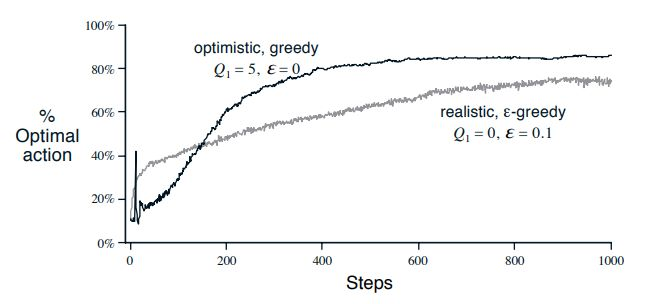
\includegraphics[width=0.9\textwidth]{images/optimistic-policy.jpg}
    \caption{Here we have prepared a testbed of 100 identical 10 armed bandits, and we test multiple strategies on this testbed. \texttt{\% Optimal Action} refers to the percentage of bandits in the testbed choosing the action with the highest value. One can see that the optimistic greedy policy sometimes outperforms realistic versions of even non-greedy algorithms.}
\end{figure}

\subsection{\texorpdfstring{The $\epsilon$-Greedy Policy}{}}
Here, our policy becomes stochastic.
\begin{eqnarray}
    A_{t} = \arg\max_{a \in A} Q_{t}(a), \text{with probability $1 - \epsilon$}\\
    A_{t} = \text{random choice from $A$}, \text{ with probability $\epsilon$}
\end{eqnarray}
Note that even in the second case, it is possible for $\arg\max_{a \in A} Q_{t}(a)$ to be chosen. All ties in the first case are broken randomly.

The advantage of this policy is that, as $t \rightarrow \infty$, $N_{t}(a) \rightarrow \infty, \forall a \in A$. If we use the sample average to estimate 
$Q_{t}$ (and if the bandit is stationary), this means that $\forall a \in A, Q_{t}(a) \rightarrow q(a)$.

If $\epsilon = 0$, then this strategy reduces to the greedy policy. For small values of $\epsilon$, the agent learns slowly, and for larger values it learns more quickly.
However, asymptotically, the agent performs better with smaller values of $\epsilon$ than with larger values.

\begin{figure}[H]
    \centering
    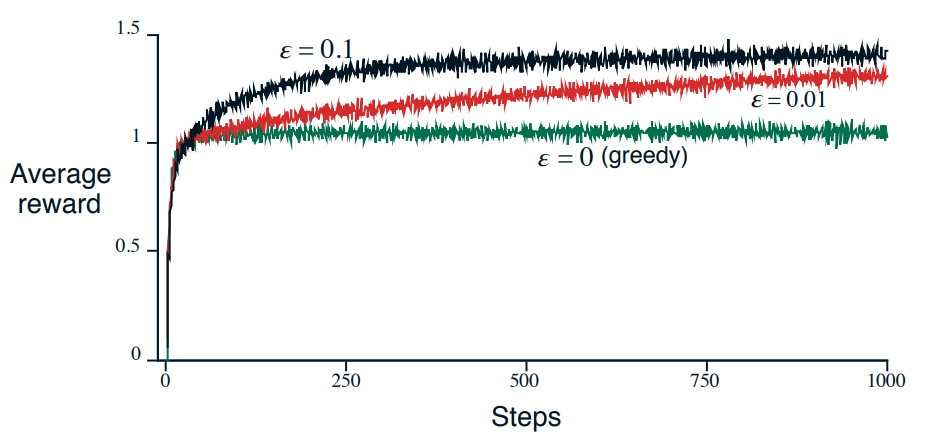
\includegraphics[width=0.9\textwidth]{images/Epsilon-greedy.png}
    \caption{We again use the same testbed described earlier and compare greedy and $\epsilon$-greedy policies. \texttt{Average Reward} here refers to the average reward each agent obtained at a particular timestep. As we can see, the $\epsilon$-greedy policies perform better than the greedy policies. Among the $\epsilon$-greedy policies, the one with the lower $\epsilon$ learns slower, but asymptotically performs better than the one with higher $\epsilon$.}
\end{figure}

\subsection{Upper Confidence Bound Action Selection}
One problem with $\epsilon$ greedy policies are that, during exploration, it gives no preference to actions with higher values, or to relatively underexplored actions over low value, well explored actions.
The UCBA selection method chooses the action with the largest upper confidence bound, where the upper confidence bound of an action is the largest value of $q(a)$ that we are reasonably confident is possible for the action $a$.
For actions tried many times, this upper bound will be close to the estimated $Q_{t}$, whereas for untried actions it'll be much larger than it. Formally, speaking the policy is:
\begin{equation}
    A_{t} = \arg\max_{a \in A}\left[Q_{t}(a) + c\sqrt{\frac{\ln t}{N_{t}(a)}}\right]
\end{equation}
When $N_{t}(a)$ is $0$, we set the argument to $\infty$. The reason we keep the additive term proportional to $\frac{1}{\sqrt{N_{t}(a)}}$ is because of the Law of Large Numbers, 
which states that the uncertainty in an estimate after $n$ measurements is proportional to $\frac{1}{\sqrt{n}}$. The $\sqrt{\ln t}$ term appears because that is a function that, although grows extremely slowly,
is unbounded. This ensures that as $t \rightarrow \infty$, $N_{t}(a) \rightarrow \infty, \forall a \in A$. 

The UCBA policy is one of the most effective ways of dealing with stationary bandits\footnote{This is because it can be shown the total regret with the UCBA policy at the $t^{th}$ timestep grows as $O(\log t)$. Here the regret at a particular move is defined as $\max(q(a), a \in A) - q(A_{t})$.}, however, it does not generalize very well
to non-stationary bandits. 
\begin{figure}[h!]
    \centering
    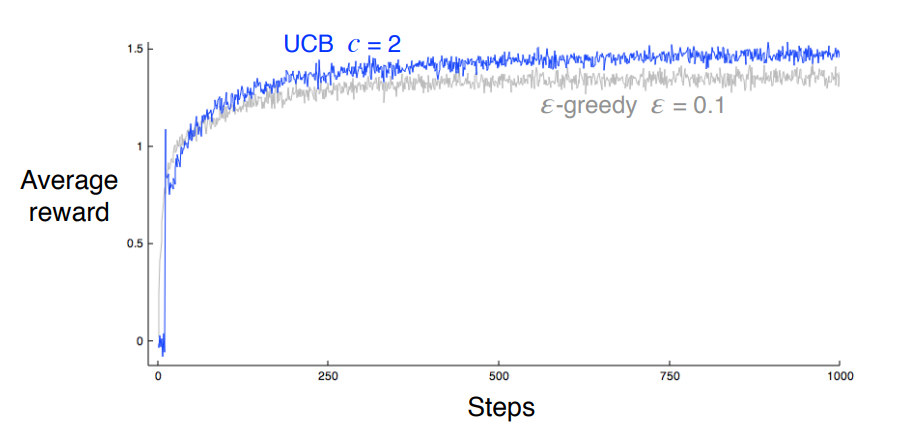
\includegraphics[width=0.7\textwidth]{images/UCBA.png}
    \caption{We use the same testbed again to compare the UCBA and $\epsilon$-greedy policies. As you can see, the UCBA policy is better.}
\end{figure}

\subsection{Gradient Bandits}
Here we associate to each action a preference $H_{t}(a)$, such that the policy becomes:
\begin{equation}
    \mathop{\mathbb{P}}(A_{t} = a) = \pi_{t}(a) = \frac{\exp{H_{t}(a)}}{\sum\limits_{b \in A} \exp{H_{t}(b)}}, \forall a \in A
\end{equation}
This distribution is known as the Softmax distribution. We try to find the values of $H_{t}(a)$ that maximize $\mathop{\mathbb{E}}_{A_{t}}\left[\mathop{\mathbb{E}}_{R | A_{t}}\left[R\right]\right] = \mathop{\mathbb{E}}_{A_{t}}\left[q(A_{t})\right]$ (the expected reward at each timestep). 
We find the optimal values of $H_{t}(a)$ via Gradient Ascent.
\begin{equation}
    H_{t + 1}(a) = H_{t}(a) + \alpha \frac{\partial}{\partial H_{t}(a)} \mathop{\mathbb{E}}_{A_{t}}\left[\mathop{\mathbb{E}}_{R | A_{t}}\left[R\right]\right]
\end{equation}

However, we cannot calculate this derivative directly as we do not know the value of $\mathop{\mathbb{E}}_{R | A_{t}}\left[R\right] = q(A_{t})$. However, it can be shown that
\begin{equation}
    \mathop{\mathbb{E}}_{A_{t}}\left[\mathop{\mathbb{E}}_{R | A_{t}}\left[R - \overline{R_{t}}\right](\mathop{\mathbb{I}}(a = A_{t}) - \pi_{t}(a))\right] = \frac{\partial}{\partial H_{t}(a)}\mathop{\mathbb{E}}_{A_{t}}\left[\mathop{\mathbb{E}}_{R | A_{t}}\left[R\right]\right]
\end{equation}
where $\mathop{\mathbb{I}}$ is the indicator function, which is $1$ if it's argument is true, and $0$ if it is false, and $\overline{R_{t}}$ is the average reward obtained so far, ie
\begin{equation}
    \overline{R_{t}} = \frac{\sum\limits_{i = 1}^{t - 1} R_{i}}{t - 1}
\end{equation}

Therefore, we can use Stochastic Gradient Ascent, where
\begin{equation}
    H_{t + 1}(a) = H_{t}(a) + \alpha (R_{t} - \overline{R_{t}})(\mathop{\mathbb{I}}(a = A_{t}) - \pi_{t}(a)), \forall a \in A
\end{equation}
where $A_{t}$ is the chosen action and $R_{t}$ is the obtained reward.

Equation (2.12) remains valid if $\overline{R_{t}}$ is replaced by any constant $X_{t}$. However, putting $X_{t} = \overline{R_{t}}$ improves the performance of the algorithm greatly by improving the speed of convergence of the gradient ascent and ensuring that below average rewards are punished immediately, as we can see in the following graph.
\begin{figure}[H]
    \centering
    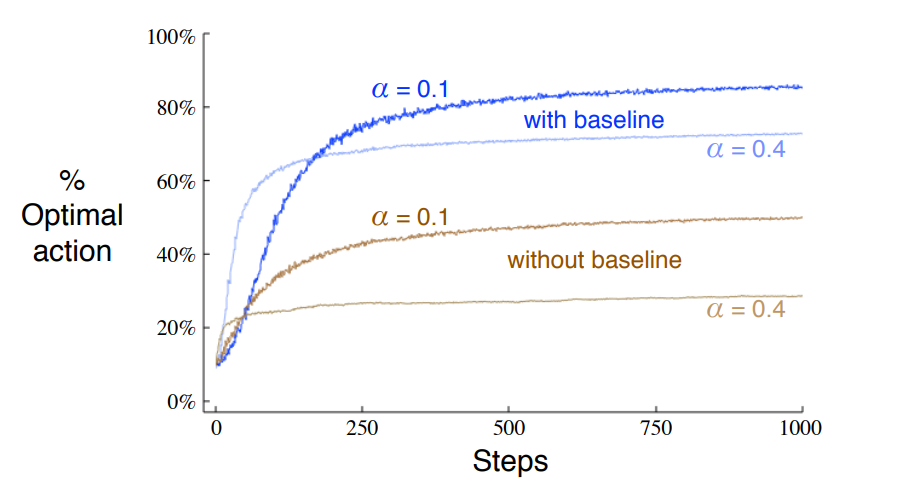
\includegraphics[width=0.7\textwidth]{images/gradient-bandit.png}
    \caption{We use the previously discussed testbed to compare different types of Gradient Ascent algorithms.}
\end{figure}

\subsection{Thompson Sampling}
This is a Bayesian approach to the multiarmed bandit problem. It can be used when the class of the reward distributions for the actions is known or can be reasonably guessed.
We assume that $R(a) \sim P(R; \theta_{a})$, ie, the rewards for each action are drawn from the same family of probability distributions, differing only in parameter $\theta$.

We use Baye's Theorem to get the posterior distribution of $\theta_{a}$ for each $a \in A$, assuming a suitable prior (usually the conjugate prior, to make our calculations easier)
\begin{equation}
    P(\theta_{a} | R_{1}, R_{2} \dots) = \frac{P(R_{1}, R_{2} \dots | \theta_{a})P(\theta_{a})}{P(R_{1}, R_{2} \dots)}
\end{equation}
We then sample\footnote{We sample $\theta$ instead of estimating it from the posterior as estimating can make this policy too greedy} $\theta^{*}_{a}$ from each posterior distribution. We then choose the action with the highest value ($\mathop{\mathbb{E}}_{\theta^{*}_{a}}\left[R\right]$), where the values are calculated according to the 
sampled parameters.

This policy is often even more efficient then the UCBA policy, as this - like the UCBA policy - focuses exploration on actions that are nearly optimal, or actions with a high variance.

A disadvantage of this method is that it is more computationally expensive than the others discussed so far.

\section{Comparing Policies}
Note that all of these policies have parameters that change the effectiveness of the policies. For each policy it is the case that the parameters have optimal values that make the policies as optimal as possible.
Considering the policies with their parameters optimized, it seems that for stationary bandits, the Upper Confidence Bound Action (UCBA) Selection Policy\footnote{This may be because it can be shown the total regret with the UCBA policy at the $t^{th}$ timestep grows as $O(\log t)$. Here the regret at a particular move is defined as $\max(q(a), a \in A) - q(A_{t})$.} and Thompson Sampling\footnote{Not shown in this graph} perform the best. 

\begin{figure}[h!]
    \centering
    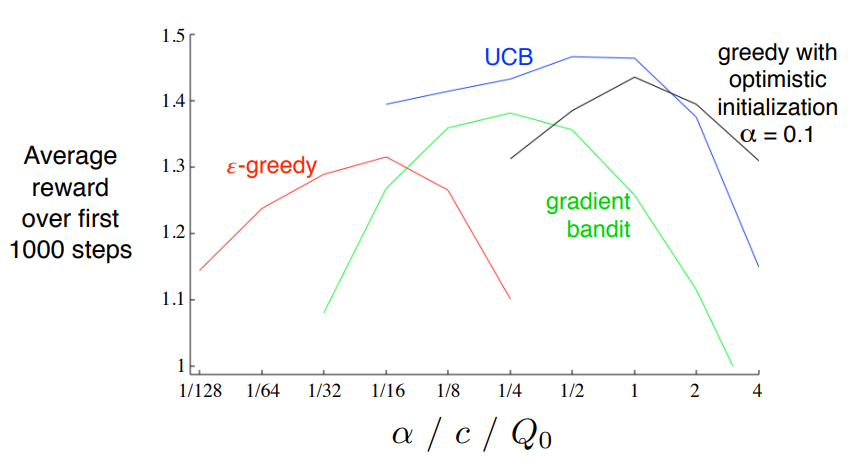
\includegraphics[width=0.9\textwidth]{images/compare-bandit.png}
    \caption{We compare all the different policies on our testbed over different values for their parameters. $\texttt{Average Reward}$ here refers to the average reward obtained over the first $1000$ timesteps. The characteristic inverted U shape of these curves shows that an optimal value exists for the parameters.}
\end{figure}

However, among these policies, only the $\epsilon$-greedy policies and the gradient bandit policies can be readily generalized to more complex RL problems.

\section{Contextual Bandits}
One of the defining properties of bandits were that they possess only one state. The situation is therefore \textbf{non-associative} (ie we don't deal with multiple states), and therefore we could easily design 
and test algorithms that balance exploration and exploitation.

When we define contextual bandits, we remove the restriction that there is only one state but still impose that the actions taken by the agent do not affect the next state of the bandit. In this case, we can train separate RL algorithms 
over each state of the bandit.

For example, say we have $k$ normal bandits. Each time we take an action on a bandit, the bandit is replaced with a different one, in a manner that is \textbf{independent} of the action taken. Also, the bandits are \textbf{distinguishable}, 
ie, before we take an action we know which bandit we are dealing with. This situation behaves exactly like a contextual bandit with $k$ states. In this scenario we can learn a separate policy for each bandit.

The conditions of \textbf{independence} and \textbf{distinguishability} allow us to decouple this problem into $k$ single state problems.

\chapter{Markov Decision Processes}
\section{Formalization of the Reinforcement Learning Problem}
Here, we will formalize the Reinforcement Learning problem we have stated informally so far, ie, where an agent selects an action based on the state of the environment in order to maximize the cumulative reward it recieves.

We assume the agent and the environment interact with each other in discrete time steps $t = 0, 1, 2 \dots$. At each time step, the agent recieves the state of the environment ($S_{t} \in S$) and makes a choice ($A_{t} \in A(S_{t})$) based on that state 
and earns a reward $R_{t + 1}$\footnote{$R_{t}$ represents the reward before the $t^{th}$ timestep. We set $R_{0} = 0$ by convention.} and transitions to state $S_{t + 1}$. 

The agent follows a policy $\pi$, where $\pi(a | s) = \mathop{\mathbb{P}}(A_{t} = a | S_{t} = s)$\footnote{In general, the agents policy will be a function of time, $\pi_{t}(a | s) = \mathop{\mathbb{P}}(A_{t} = a | S_{t} = s)$ which changes as the agent learns. However, we assume the agent 
has a stationary policy in order to calculate certain values associated with each state. After each timestep, we will use these values (calculated with the old policy) to update our policy. Towards the end our policy will reach a stationary optimal policy.}. Our agent must learn the optimal policy.

\section{Return and Discounting}
However, we have not yet formally defined what it is that we must optimize. So far we have been talking about optimizing the expected cumulative reward $R_{t + 1} + R_{t + 2} + \dots$. However, for tasks that do not terminate eventually, this becomes an infinite sum, which may not converge.
Therefore, we define a quantity known as the return $G_{t}$ in different ways for different tasks. It is the expected return $\mathop{\mathbb{E}}(G_{t})$ that the agent seeks to maximize at each timestep.

Tasks that always terminate after a finite number of timesteps are known as episodic tasks. For such tasks, we can define $G_{t}$ as the cumulative reward obtained from the $t^{th}$ timestep onwards.
\begin{equation}
    G_{t} = \sum\limits_{k = 0}^{T - k - 1} R_{t + k + 1}
\end{equation}

For non-episodic tasks however, this sum may not converge. Therefore, we introduce the concept of discounting, where we value rewards obtained later less than those obtained sooner. To be precise, we define $G_{t}$ as:
\begin{equation}
    G_{t} = \sum\limits_{k = 0}^{\infty} \gamma^{k}R_{t + k + 1}
\end{equation}
where $0 \leq \gamma \leq 1$. If $\gamma < 1$ and the rewards are bounded then this sum will always converge. $G_{t}$ will satisfy the recurrence $G_{t} = R_{t + 1} + \gamma G_{t + 1}$ (this recurrence will prove useful later on).

$\gamma$ is known as the \textit{discount rate}, and determines how far sighted our agent is. If $\gamma = 0$, then our 
agent is said to be greedy (or) myopic, as in this $\mathop{\mathbb{E}}(G_{t}) = \mathop{\mathbb{E}}(R_{t + 1})$, and therefore the optimal policy would be to choose the action with the highest expected reward without worrying about future rewards.

We can unify the notation for episodic and non-episodic tasks by having the terminal states of episodic tasks have only a single action, that always gives $0$ reward and never changes the state of the environment.
We can then define the return for all tasks using equation (3.2), with $\gamma = 1$ for episodic tasks. Note that for episodic tasks, if $S_{t}$ is a terminal state, $G_{t} = 0$.

\section{Markov Decision Processes and the Markov Property}
The current state should provide enough information to determine the probability distributions of the rewards and the transition probabilities to the next state (given the next state). At the most it can contain an entire description of the history of the environment 
upto the present moment. This is quantified mathematically by saying the states and rewards must satisfy the \textit{Markov Property}, ie 
\begin{equation}
    \mathop{\mathbb{P}}(S_{t + 1} = s, R_{t + 1} = r | S_{t}, A_{t}, R_{t}, S_{t - 1}, A_{t - 1} \dots) = \mathop{\mathbb{P}}(S_{t + 1} = s, R_{t + 1} = r | S_{t}, A_{t})
\end{equation}
for all $r$, $s \in S$. This means that the distributions of the rewards and the next state depend only on the current state and the action chosen.

For notational convenience, we will use $p(r, s' | s, a)$ to denote this distribution, ie 
\begin{equation}
    p(s', r | s, a) = \mathop{\mathbb{P}}(S_{t + 1} = s', R_{t + 1} = r | S_{t} = s, A_{t} = a)
\end{equation}

We say a task is a \textit{complete-knowledge} task if the distribution $p(s', r | s, a)$ is known before hand, and an \textit{incomplete-knowledge} task if it is unknown, and must be learnt by the agent.

$p(s', r | s, a)$ along with the set of states $S$, set of actions for each state $A(s)$ (for $s \in S$) completely specifies the task at hand. Tasks that can be formulated this way in terms of 
states and actions are known as \textbf{Markov Decision Processes}. Along with the agents policy $\pi(s | a)$, the entire interaction between the Agent and the Environment is specified.

We can define $R_{sa}$ as the expected reward given a state-action pair.
\begin{equation}
    R_{sa} = \mathop{\mathbb{E}}\left[R_{t + 1} | S_{t} = s, A_{t} = a\right] = \sum\limits_{r, s' \in S} r p(s', r | s, a)
\end{equation}
The state transition probability $P_{ss'}^{a}$ is defined as the probability of transitioning from state $s$ to state $s'$ given action $a$ was chosen.
\begin{equation}
    P_{ss'}^{a} = \mathop{\mathbb{P}}(S_{t + 1} = s' | S_{t} = s, A_{t} = a) = \sum\limits_{r} p(s', r | s, a)
\end{equation}
We can also define $R_{ss'}^{a}$ as the expected reward given a triplet of the current state $s$, the chosen action $a$, and the next state $s'$.
\begin{equation}
    R_{ss'}^{a} = \mathop{\mathbb{E}}\left[R_{t + 1} | S_{t} = s, S_{t + 1} = s', A_{t} = a\right] = \frac{\sum\limits_{r} r p(s', r | s, a)}{\sum\limits_{r} p(s', r | s, a)}
\end{equation}

We can diagramatically represent Markov Decision Processes via Transition Diagrams, which are directed multigraphs in which each node represents a state, and between every two nodes representing states 
$s, s' \in S$, there is an edge from node $s$ to node $s'$ for each action $a \in A(s)$. These edges are associated with the state transition probabilities $P_{ss'}^{a}$ and the expected rewards $R_{ss'}^{a}$.
The sum of $P_{ss'}^{a}$ for all edges leaving a node $s$ is always $1$.

\section{The Bellman Equations}
For every state $s$ in the MDP, we can define it's value under the policy $\pi$ as 
\begin{equation}
    v_{\pi}(s) = \mathop{\mathbb{E}}\left[G_{t} | S_{t} = s\right]
\end{equation}
$v_{\pi}$ is known as the state-value function.

We can also define $q_{\pi}$ (known as the action-value function) as 
\begin{equation}
    q_{\pi}(s, a) = \mathop{\mathbb{E}}\left[G_{t} | S_{t} = s, A_{t} = a\right]
\end{equation}

From the total probability theorem, we can conclude that 
\begin{equation}
    v_{\pi}(s) = \sum\limits_{a \in A(s)} q_{\pi}(s, a)\pi(a | s)
\end{equation}

Now, we can also find $q_{\pi}$ in terms of $v_{\pi}$.
\begin{equation}
    q_{\pi}(s, a) = \mathop{\mathbb{E}}\left[G_{t} | S_{t} = s, A_{t} = a\right] = \mathop{\mathbb{E}}\left[R_{t + 1} + \gamma G_{t + 1} | S_{t} = s, A_{t} = a\right]
\end{equation} 
Hence,
\begin{equation}
    q_{\pi}(s, a) = \sum\limits_{r, s' \in S} p(s', r | s, a)(r + \gamma \mathop{\mathbb{E}}\left[G_{t + 1} | S_{t + 1} = s', S_{t} = s, A_{t} = a\right])
\end{equation}
By the Markov Property, 
\begin{equation}
    \mathop{\mathbb{E}}\left[G_{t + 1} | S_{t + 1} = s', S_{t} = s, A_{t} = a\right] = \mathop{\mathbb{E}}\left[G_{t + 1} | S_{t + 1} = s'\right] = v_{\pi}(s')
\end{equation}
Therefore,
\begin{equation}
    q_{\pi}(s, a) = \sum\limits_{r, s' \in S} p(s', r | s, a)(r + \gamma v_{\pi}(s'))
\end{equation}

Using equations (3.10) and (3.14) we can get recursive relations for $q_{\pi}$ and $v_{\pi}$.
\begin{equation}
    q_{\pi}(s, a) = \sum\limits_{r, s' \in S} p(s', r | s, a)(r + \gamma\sum\limits_{a' \in A(s')}\pi(a' | s') q_{\pi}(s', a'))
\end{equation}
\begin{equation}
    v_{\pi}(s) = \sum\limits_{\substack{a \in A(s)\\r, s' \in S}} \pi(a | s) p(s', r | s, a)(r + \gamma v_{\pi}(s'))
\end{equation}

These equations are known as the \textbf{Bellman Equations} for the Action Value and State Value functions respectively. Using these equations, for any policy $\pi$, we can find all the $v_{\pi}(s)$ and 
$q_{\pi}(s, a)$ for all $s, a$ up assuming we know the dynamics of the MDP ($p(s', r | s, a)$). This is because we usually know the values of some states of the MDP already, or we can assign values to these 
based on some heuristic. For example, in episodic MDPs, the terminal states have $0$ value. From these states, we can work from the bottom up to find all the values.

\section{Bellman Optimality Equations}
We say a policy $\pi_{1}$ is better than a policy $\pi_{2}$ for an MDP if $\forall s \in S, v_{\pi_{1}}(s) \geq v_{\pi_{2}}(s)$ and $\forall s \in S, a \in A(S), q_{\pi_{1}}(s, a) \geq q_{\pi_{2}}(s, a)$ (note that due to equations (3.10) and (3.14) these two conditions are equivalent)\footnote{There may be policies which are not comparable, ie Now, if $v_{\pi_{1}}(s) \geq v_{\pi_{2}}(s)$ for some $s$ and $v_{\pi_{1}}(s) < v_{\pi_{2}}(s)$ for other $s$. We have defined in this way a \textit{partial order} on policies.}.
It can be shown that there will always exist an optimal policy $\pi^{*}$ that satifies $v_{\pi^{*}}(s) \geq v_{\pi}(s)$ and $q_{\pi^{*}}(s, a) \geq q_{\pi}(s, a)$, $\forall s \in S, \forall \text{ policies } \pi$. Although there may be many optimal policies, it is easy to show that $v_{\pi^{*}}$ and $q_{\pi^{*}}$ are unique\footnote{If $v_{1}$ and $v_{2}$ are the state value functions for two optimal policies, then $\forall s \in S$, $v_{1}(s) \geq v_{2}(s)$ and $v_{2}(s) \geq v_{1}(s)$.}. To show this uniqueness, we write $v_{*} = v_{\pi^{*}}$ and $q_{*} = q_{\pi^{*}}$.
Clearly, $\forall s \in S, a \in A(S)$ $q_{*}(s, a) = \max_{\pi}(q_{\pi}(s, a))$ and $v_{*}(s) = \max_{\pi}(v_{\pi}(s))$.

We can show that the optimal value functions must satisfy the following equations, which are known as the \textbf{Bellman Optimality Equations}.
\begin{equation}
    q_{*}(s, a) = \sum\limits_{r, s' \in S} p(s', r | s, a)(r + \gamma \max_{a \in A(s')} q(s', a))
\end{equation}
and
\begin{equation}
    v_{*}(s) = \max_{a \in A(s)} q_{*}(s, a) = \max_{a \in A(s)} \sum\limits_{r, s' \in S} p(s', r | s, a)(r + \gamma v_{*}(s'))
\end{equation}

We can intuitively justify this by stating that in the optimal policy we will always choose an action that leads to maximum return, ie, 
\begin{equation}
    v_{*}(s) = \max\limits_{a \in A(s)} q_{*}(s, a)
\end{equation}
Using this along with equation (3.14), we get the Bellman Optimality Equations, and we can also show that and policy $\pi$ satisfying $\pi(a | s) \neq 0$ only if $a \in \arg\max\limits_{a \in A(s)} q_{\pi}(s, a)$ is an optimal policy (the optimal policy is greedy with respect to the action value function).

A formal proof\footnote{This part is not essential reading for the project} would go as follows:
Assume we have some function $v(s)$ that satisfies
\begin{equation}
    v(s) = \max_{a \in A(s)} \sum\limits_{r, s' \in S} p(s', r | s, a) (r + \gamma v(s'))
\end{equation}
Now, clearly (by equation (3.16)) this corresponds to an action-value function for a policy $\pi$ such that $\pi(a | s) \neq 0$ only if $a \in \arg\max\limits_{a \in A(s)} \sum\limits_{r, s' \in S} p(s', r | s, a) (r + \gamma v(s'))$. 
By equation (3.14), the corresponding action value function would be $q(s, a) = \sum\limits_{r, s' \in S} p(s', r | s, a) (r + \gamma v(s'))$, ie $\pi(a | s) \neq 0$ only if $a \in \arg\max\limits_{a \in A(s)} q(s, a)$.

Now, we shall prove that $v(s) \geq v_{\pi'}(s), \forall s \in S$ for all policies $\pi'$. This  makes $\pi$ an optimal policy\footnote{This means that any deterministic policy that is greedy with respect to it's own action value function is an optimal policy, as it is trivial to show that any such policy must satify the Bellman Optimality Equations.}, which makes $v$ \textbf{the} optimal state value function.
Therefore, due to uniqueness, the optimal state value function must satisfy the equation (3.20), which is nothing but the Bellman Optimality Condition for the state value function, from which we can derive the Bellman Optimality Condition for the action value function (using equation (3.14) along with the fact that $v(s) = \max\limits_{a \in A(s)} q(s, a)$).

To prove that $v(s) \geq v_{\pi'}(s), \forall s \in S$, for all policies $\pi'$, we proceed by induction.

For the terminal states $v(s) = v_{\pi'}(s) = 0$, therefore, $v(s) \geq v_{\pi'}(s)$. Now, assume for some state $s$, every $s'$ with $p(s', r | s, a) > 0$ for some $r$ and some $a$ has $v(s') \geq v_{\pi'}(s')$.
Now,
\begin{equation}
    v(s) = \max_{a \in A(s)} \sum\limits_{r, s' \in S} p(s', r | s, a) (r + \gamma v(s')) \geq \max_{a \in A(s)} \sum\limits_{r, s' \in S} p(s', r | s, a) (r + \gamma v_{\pi'}(s'))
\end{equation}
Therefore,
\begin{equation}
    v(s) \geq \sum\limits_{\substack{a \in A(s)\\r, s' \in S}} \pi'(a | s) p(s', r | s, a) (r + \gamma v_{\pi'}(s')) = v_{\pi'}(s)
\end{equation}
Hence,
\begin{equation}
    v(s) \geq v_{\pi'}(s)
\end{equation}

Therefore, by the inductive principle $\forall s \in S, v(s) \geq v_{\pi'}(s)$. Using this, we can prove the Bellman Optimality Conditions via the method described above.

Note, that we here we have proved that the Bellman Optimality Equations impose a sufficient condition on the value functions for them to be optimal. The uniqueness of the value functions leads to this being a necessary condition as well.

\section{Solving the Bellman Optimality Conditions}
In principle, if the dynamics of the MDP ($p(s', r | s, a)$) are known (the MDP is complete knowledge), then we can solve the Bellman Optimality Equations from the bottom up, and use these to find the optimal policy, ie, we can solve the Reinforcement Learning Problem.

The two principal difficulties with this are that, often $p(s', r | s, a)$ are not known beforehand and must be learnt, and that in most situations the number of states is too large for the previously described method to be computationally feasible. Therefore, we develop various methods and 
hueristics in order to approximately solve these equations.

\chapter{Dynamic Programming}
\section{Introduction}
Dynamic Programming\footnote{The name arises due to the fact that most algorithms in this class cache the values of the states encountered instead of recomputing them each time.} Algorithms are a collection of iterative algorithms that can be used to compute the optimal policy for \textbf{complete-knowledge}\footnote{$p(s', r | s, a)$ is known to the agent.} finite MDPs. 

For complete knowledge finite MDPs, it is possible to explicitly solve the Bellman Optimality Equations to find the optimal value and action value functions. The optimal policy would then be greedy with respect to 
the optimal action value function. However, solving the Bellman Optimality Equations explicitly may be computationally infeasible, especially when the number of possible states is extremely large. Hence, we develop 
methods that iteratively converge to the Optimal Policy\footnote{An analogy with Gradient Descent may be made here. This analogy can be extended further as we discuss variations on Dynamic Programming.}.

Broadly speaking, this class of algorithms starts out with an arbitrarily chosen policy and value function. The value function is then made to fit the policy more accurately, after which the policy is changed to be 
greedy with respect to this value function. This process will eventually converge to the optimal policy and value functions for the MDP\footnote{Note that the optimal policy and value functions are fixed points of this algorithm, as the optimal policy is greedy with respect to it's own value function.}.

\section{Policy Evaluation}
Policy Evaluation refers to a class of algorithms that can be used to find the value functions for a given policy $\pi$. This can also be done explicitly by solving the Bellman Equations, but, as mentioned earlier, this becomes 
computationally infeasible when the number of possible states ($\left|S\right|$) is extremely large. Therefore, here too we use iterative algorithms that converge to the actual value functions.

These algorithms function by converting the Bellman Equations into update rules. We start with a guess value function $v_{0}$\footnote{Note that the $v_{0}(s)$ must be $0$ for all terminal states $s$. This ensures that $v_{k}(s) = 0, \forall s \in S^{T}$. This basically means our initial guess must follow the boundary conditions that $v_{\pi}$ follow $\forall \pi$.}. We then repeatedly apply the following update rule:
\begin{equation}
    v_{k + 1}(s) = \sum\limits_{\substack{a \in A(s)\\r, s' \in S}} \pi(a | s) p(s', r | s, a) (r + \gamma v_{k}(s')), \forall s \in S
\end{equation}

It can be shown that $\lim\limits_{k \rightarrow \infty} v_{k} = v_{\pi}$. Note, that $v_{\pi}$ itself is a fixed point of this update rule (it remains unchanged by this update), due to the Bellman Equations. This algorithm 
is known as iterative policy evaluation. Once we find $v_{\pi}$, we can find $q_{\pi}$ via the Bellman Equations:
\begin{equation}
    q_{\pi}(s, a) = \sum\limits_{r, s' \in S} p(s', r | s, a)(r + \gamma\sum\limits_{a' \in A(s')}\pi(a' | s') q_{\pi}(s', a'))
\end{equation}

It is also possible to iteratively find $q_{\pi}$ instead of $v_{\pi}$ using it's Bellman Equation as an update rule, ie we start with an initial guess $q_{0}$, and update it according to:
\begin{equation}
    q_{k + 1}(s, a) = \sum\limits_{r, s' \in S} p(s', r | s, a)(r + \gamma\sum\limits_{a' \in A(s')}\pi(a' | s') q_{k}(s', a'))
\end{equation}
Here also $\lim\limits_{k \rightarrow \infty} q_{k} = q_{\pi}$, and we can therefore find $v_{\pi}$ using $v_{\pi}(s) = \sum\limits_{a \in A(s)} \pi(a | s) q_{\pi}(s, a)$. This algorithm is less efficient than the previously described one, as during each update we must iterate over the space of states and the space of actions ($S \times A$), rather than $S$ alone.

Each update to the value of a state $s$ is known as a backup to $s$. We can do our backups in-place, ie, once we calculate the new value of $v(s)$ via the update rule, we immediately use this new value to update $v(s')$ for other states $s'$. This generally leads to faster convergence as we use the updated information as soon as it becomes available.
Since, in this algorithm, to go from $v_{k}$ to $v_{k + 1}$, we update $v(s)$ for every state $s$, this update is known as a full backup. Full backups run in $O(\left|S\right|^{2})$ and therefore can be extremely computationally expensive. \textit{Asynchronous Dynamic Programming} and \textit{Generalized Policy Iteration} techniques (discussed later) provide ways for us to manage this cost.


\section{Policy Improvement}
We can use the computed value functions to improve our policy. This is done by changing our policy to be greedy with respect to the newly computed value function, ie 
\begin{equation}
    \pi'(s) = \arg\max\limits_{a \in A(s)} q_{\pi}(s, a)
\end{equation}
with ties broken arbitrarily\footnote{Note that $\pi'$ here is a deterministic policy, ie, $\mathop{\mathbb{P}}(A_{t} = a | S_{t} = s)$ is $1$ for $a = \pi'(s)$ and $0$ for all other $a \in A(s)$. We abuse notation for deterministic policies by using $\pi$ to stand for both $\mathop{\mathbb{P}}(A_{t} = a | S_{t} = s)$ ($\pi(a | s)$) and for the action that is chosen ($\pi(s)$).}.

This new policy will be better than (or at least as good as) the previous policy. This can be formalized via the \textit{Policy Improvement Theorem}.
\subsection{The Policy Improvement Theorem}
The statement of the theorem is as follows:

If $\pi$ and $\pi'$ are two policies such that
\begin{equation}
    \mathop{\mathbb{E}}_{a \sim \pi'}\left[q_{\pi}(s, a)\right] \geq v_{\pi}(s), \forall s \in S
\end{equation}
then
\begin{equation}
    v_{\pi'}(s) \geq v_{\pi}(s), \forall s \in S
\end{equation}
ie, $\pi'$ is at least as good a policy as $\pi$. 

The proof of this theorem is as follows:

Firstly, note that $\mathop{\mathbb{E}}_{a \sim \pi'}\left[q_{\pi}(s, a)\right] = \sum\limits_{a \in A(s)} \pi'(a | s) q_{\pi}(s, a)$. Therefore, our inequality becomes
\begin{equation}
    \sum\limits_{a \in A(s)} \pi'(a | s) q_{\pi}(s, a) \geq v_{\pi}(s), \forall s \in S
\end{equation}

Our proof is by induction. Note that for all terminal states $s$, $v_{\pi'}(s) = v_{\pi}(s) = 0$. For some state $s$, assume that every $s'$ with $p(s', r | s, a) > 0$ for some $r, a$ has $v_{\pi'}(s') \geq v_{\pi}(s')$.
Now,
\begin{equation}
    v_{\pi'}(s) = \sum\limits_{\substack{a \in A(s)\\r, s' \in S}} \pi'(a | s) p(s', r | s, a) (r + \gamma v_{\pi'}(s'))
\end{equation}
Since, $v_{\pi'}(s') \geq v_{\pi}(s')$
\begin{equation}
    v_{\pi'}(s) \geq \sum\limits_{\substack{a \in A(s)\\r, s' \in S}} \pi'(a | s) p(s', r | s, a) (r + \gamma v_{\pi}(s'))
\end{equation}
The RHS here can be rewritten as $\sum\limits_{a \in A(s)} \pi'(a | s) \sum\limits_{r, s' \in S} p(s', r | s, a) (r + \gamma v_{\pi}(s'))$ which is nothing but $\sum\limits_{a \in A(s)} \pi'(a | s) q_{\pi}(s, a)$.

Therefore,
\begin{equation}
    v_{\pi'}(s) \geq \sum\limits_{a \in A(s)} \pi'(a | s) q_{\pi}(s, a) \geq v_{\pi}(s)
\end{equation}
Hence, $v_{\pi'}(s) \geq v_{\pi}(s)$. By induction, this means that $v_{\pi'}(s) \geq v_{\pi}(s), \forall s \in S$.

\subsection{Improving our Policy}
If we change our policy in the manner described earlier, ie 
\begin{equation}
    \pi'(s) = \arg\max\limits_{a \in A(s)} q_{\pi}(s, a), \forall s \in S
\end{equation}
then for all states $s$,
\begin{equation}
    \mathop{\mathbb{E}}_{a \sim \pi'}\left[q_{\pi}(s, a)\right] = \max\limits_{a \in A(s)} q_{\pi}(s, a) \geq \sum\limits_{a \in A(s)} \pi(a | s) q_{\pi}(s, a) = v_{\pi}(s)
\end{equation}
and therefore, by the Policy Improvement Theorem,
\begin{equation}
    v_{\pi'}(s) \geq v_{\pi}(s), \forall s \in S
\end{equation}
ie, $\pi'$ is at least as good as $\pi$.

If $\pi'$ is exactly as good as $\pi$, ie 
\begin{equation}
    v_{\pi'}(s) = v_{\pi}(s), \forall s \in S
\end{equation}
then the inequality in equation (4.12) must be an equality. Therefore, 
\begin{equation}
    v_{\pi}(s) = \max\limits_{a \in A(s)} q_{\pi}(s, a) = \max\limits_{a \in A(s)} \sum\limits_{r, s' \in S} p(s', r | s, a)(r + \gamma v_{\pi}(s'))
\end{equation}
ie, $v_{\pi}$ (and therefore $v_{\pi'}$) both satisfy the Bellman Optimality Equations, and therefore both $\pi$ and $\pi'$ are optimal policies.

This means that, given the value function of a policy, we can modify the policy in such as a way as to make it strictly better, unless it is already an optimal policy (in which case it can only change to another optimal policy).

This leads to the idea of \textit{policy iteration}.
\section{Policy Iteration}
Policy Iteration refers to a class of algorithms that alternate Policy Evaluation and Policy Improvement in order to find the optimal policy for the MDP.

We start with an arbitrary policy $\pi_{0}$, and compute it's value function $v_{\pi_{0}}$ via policy evaluation. The update rule we then follow is:
\begin{itemize}
    \item Given value function $v_{\pi_{k - 1}}$, get policy $\pi_{k}$ that is greedy with respect to $v_{\pi_{k - 1}}$ by policy improvement.
    \item Given policy $\pi_{k}$, compute $v_{\pi_{k}}$ via policy evaluation.
\end{itemize}
We keep doing this until we reach an optimal policy $\pi_{*}$, which occurs when there is no improvement in the policy between the $k^{th}$ and $(k + 1)^{th}$ iterations.

Doing this, we get a monotonically increasing sequence of policies and value functions during policy iteration which eventually converges to an optimal policy and the optimal value function.
\begin{equation*}
    \pi_{0} \xrightarrow[]{\text{E}} v_{\pi_{0}} \xrightarrow[]{\text{I}} \pi_{1} \xrightarrow[]{\text{E}} v_{\pi_{1}} \xrightarrow[]{\text{I}} \pi_{2} \xrightarrow[]{\text{E}} v_{\pi_{2}} \dots \xrightarrow[]{\text{I}} \pi_{*} \xrightarrow[]{\text{E}} v_{*}
\end{equation*}

However, Policy Iteration can be extremely computationally intensive, as it involves multiple iterations of policy evaluation, each of which involves multiple iterations of full backups, each of which involves a traversal of over each possible state of the MDP. 

Therefore, we develop methods to reduce the amount of computation we need to do. One such method is \textit{value iteration}.

\section{Value Iteration}
The key idea in value iteration is that we don't need to find the exact value function $v_{\pi_{k}}$ in order to get an improvement by making our new policy greedy with respect to the value function. We can just do a few full backups and then move on to policy improvement.

In value iteration, we do exactly one full backup, and move on to the policy improvement step immediately afterwards. The update rules then become:
\begin{equation}
    v_{k + 1}(s) = \max\limits_{a \in A(s)} \sum\limits_{r, s' \in S} p(s', r | s, a) (r + \gamma v_{k}(s'))
\end{equation}
where, at every iteration, $\pi_{k}(s) = \arg\max\limits_{a \in A(s)} \sum\limits_{r, s' \in S} p(s', r | s, a) (r + \gamma v_{k}(s'))$.

Note, that equation (4.16) is nothing but the Bellman Optimality Condition converted into an update rule, and therefore the optimal value function will be a fixed point of this update rule.
\section{Asynchronous Dynamic Programming}
Sometimes, for large state spaces, the cost of doing even a single full backup every iteration may be too large. In these situations, it is often the case that the most states are very unlikely to occur in the agent's experience of playing the game. 
Therefore, in asynchronous dynamic programming, we update only a subset of the states\footnote{An analogy may be drawn with stochastic gradient descent here.}, ideally the ones that are most relevant. 

Asynchronous Dynamic Programming is often done by training the agent while it is experiencing the MDP. We backup only the states that the agent has encountered so far. This causes learning to be focused on the most relevant states.
\section{Generalized Policy Iteration}
Starting from Policy Iteration, our strategy to find the optimal policy has been to both update the value function for the states (policy evaluation) and to update the policy to make it greedy with respect to the current value function (policy improvement). Such algorithms are known as 
Generalized Policy Iteration algorithms. To make these algorithms less computationally intensive we have spread the policy evaluation around and intermixed it more with policy improvement. This allows us to not have to wait for long policy evaluations in order to improve our policy.

All Generalized Policy Iteration algorithms will eventually converge to an optimal policy, as, by the Bellman Optimality Equations, these policies are greedy with respect to their own value functions.

% \section{Itemization in Unordered Lists}
% The same thing, but as an unordered list.
% \begin{itemize}
%     \item Comparison based sorting algorithms\\
%           These algorithms will always have $\Omega(n\log n)$ comparisons.
%           \begin{itemize}
%               \item Sorting algorithms that are $O(n^2)$ on average
%                     \begin{itemize}
%                         \item Bubble Sort
%                         \item Insertion Sort
%                         \item Selection Sort
%                         \item Comb Sort
%                         \item Exchange Sort
%                         \item Shell Sort
%                     \end{itemize}
%               \item Sorting algorithms that are $O(n\log n)$ on average
%                     \begin{itemize}
%                         \item Merge Sort
%                         \item Heap Sort
%                         \item Quick Sort
%                     \end{itemize}
%           \end{itemize}
%     \item Distribution based sorting algorithms\\
%           These algorithms can be more efficient than $n\log n$ and are all $\Omega(n)$.\\
%           However they make some assumptions about the distribution of the elements of the array.
%           \begin{itemize}
%               \item Counting Sort\\
%                     Here it is assumed that the elements of the array belong to a set $S$ of possibilities.\\
%                     It's time complexity is then $O(n + |S|)$.
%               \item Bucket Sort\\
%                     Here we divide the array into $k$ buckets, and sort the buckets, and then merge them.\\
%                     It's time complexity is $O(n + \frac{n^{2}}{k} + k)$.
%               \item Radix Sort\\
%                     Here we assume that the elements are to be sorted lexicographically.\\
%                     It's time complexity is $O(wn)$ where $w$ is the length of each element.
%           \end{itemize}
% \end{itemize}


% % \chapter{Images with Captions}
% % Have a look at these images with captions related to sorting.
% % \begin{figure}[h!]
% %     \centering
% %     % \includegraphics[width=0.6\textwidth]{images/selection-sort.png}
% %     \caption{Selection Sort}
% % \end{figure}
% % \begin{figure}[h!]
% %     \centering
% %     % \includegraphics[width=0.8\textwidth]{images/complexities.png}
% %     \caption{Time Complexities of some Sorting Algorithms}
% % \end{figure}

% \chapter{A Table with Captions}

% \begin{table}[h!]
%     \begin{tabular}{ |p{2.5cm}||p{2.5cm}|p{2.5cm}|p{2.5cm}|p{2.5cm}|  }
%         \hline
%         \multicolumn{5}{|c|}{Sorting Algorithms} \\
%         \hline
%         \centering Algorithm& \centering Best Case Complexity & \centering Average Case Complexity&\centering Worst Case Complexity& Memory Complexity\\
%         \hline
%         \centering Bubblesort & \centering $\Omega(n)$ & \centering $\Theta(n^{2})$ & \centering $O(n^{2})$ & $O(1)$\\
%         \hline
%         \centering Insertion Sort & \centering $\Omega(n)$ & \centering $\Theta(n^{2})$ & \centering $O(n^{2})$ & $O(1)$\\
%         \hline
%         \centering Selection Sort & \centering $\Omega(n^{2})$ & \centering $\Theta(n^{2})$ & \centering $O(n^{2})$ & $O(1)$\\
%         \hline
%         \centering Comb Sort & \centering $\Omega(n\log n)$ & \centering $\Theta(n^{2})$ & \centering $O(n^{2})$ & $O(1)$\\
%         \hline
%         \centering Exchange Sort & \centering $\Omega(n^{2})$ & \centering $\Theta(n^{2})$ & \centering $O(n^{2})$ & $O(1)$\\
%         \hline
%         \centering Shell Sort & \centering $\Omega(n\log n)$ & \centering $\Theta(n^{\frac{4}{3}})$ & \centering $O(n^{\frac{3}{2}})$ & $O(1)$\\
%         \hline
%         \centering Merge Sort & \centering $\Omega(n\log n)$ & \centering $\Theta(n\log n)$ & \centering $O(n\log n)$ & $O(n)$\\
%         \hline
%         \centering Heap Sort & \centering $\Omega(n\log n)$ & \centering $\Theta(n\log n)$ & \centering $O(n\log n)$ & $O(1)$\\
%         \hline
%         \centering Quick Sort & \centering $\Omega(n\log n)$ & \centering $\Theta(n\log n)$ & \centering $O(n^{2})$ & $O(\log n)$\\
%         \hline
%         \centering Counting Sort & \centering $\Omega(n + r)$ & \centering $\Theta(n + r)$ & \centering $O(n + r)$ & $O(n + r)$\\
%         \hline
%         \centering Bucket Sort & \centering $\Omega(n + r)$ & \centering $\Theta(n + r)$ & \centering $O(n + r)$ & $O(n + r)$\\
%         \hline
%         \centering Radix Sort & \centering $\Omega(n)$ & \centering $\Theta(n\frac{k}{d})$ & \centering $O(n\frac{k}{d})$ & $O(n + 2^{d})$\\
%         \hline
%     \end{tabular}
%     \caption{Some popular sorting algorithms and their complexities}
% \end{table}

% \chapter{Algorithm and Code}
% Here we will discuss an algorithm to print the first $n$ Fibonacci numbers.
% This was part of the second inlab of \textbf{CS 251}.
% The pseudocode of this algorithm is as follows:
% \begin{algorithmic}[1]
%     \State $x \gets 0$
%     \State $y \gets 1$
%     \For{$k \gets 1$ to $n$}
%     \State \textbf{print} $x$
%     \State $temp \gets x$
%     \State $x \gets y$
%     \State $y \gets y + temp$
%     \EndFor
% \end{algorithmic}
% The implementation of this algorithm as a \textit{Bash} Script is as follows:

% \begin{lstlisting}[language=bash,caption={Calculating the Fibonacci Numbers}]
% #! /bin/bash

% x=0
% y=1
% str=""
% num=$(($1))
% for ((i=0; i<$num; i++))
% do
%     str+="$x "
%     temp=$(($x))
%     x=$(($y))
%     y=$(($y+$temp))
% done
% echo $str
% \end{lstlisting}

% \chapter{Minipage}
% The following is a boxed minipage.\\
% \fbox{
%     \begin{minipage}{6cm}
%         Lorem ipsum dolor sit amet, consectetur adipiscing elit,
%         sed do eiusmod tempor incididunt ut labore et dolore magna aliqua.\\ 
%         Ut enim ad minim veniam, quis nostrud exercitation ullamco laboris nisi ut aliquip ex ea commodo consequat.\\
%         Duis aute irure dolor in reprehenderit in voluptate velit esse cillum dolore eu fugiat nulla pariatur.\\
%         Excepteur sint occaecat cupidatat non proident, sunt in culpa qui officia deserunt mollit anim id est laborum.
%     \end{minipage}
% }

\end{document}